\documentclass[12pt]{article}
\usepackage{../../lecture_notes}
\usepackage{../../math}
\usepackage{../../uark_colors}

\hypersetup{
  colorlinks = true,
  allcolors = ozark_mountains,
  breaklinks = true,
  bookmarksopen = true
}

\begin{document}
\begin{center}
  {\Huge\bf Review Notes}
  
  \smallskip
  {\large\it ECON 4753 — University of Arkansas}

  \medskip
  {\large Prof. Kyle Butts}
\end{center}

\part{Review of Algebra}

\section{Summation}

When working with data, it is common to have many observations. We want to have a notation that lets us work with all of those observations at once. Let's say we have some set of observations for some variable $x$. We can write them out as $x_1, x_2, \dots, x_n$ where the subscript denotes which of the $n$ observations we are referring too.

The first example of this is trying to sum up the value of a variable for all observations. We could write $x_1 + x_2 + \dots + x_n$ to represent summing up all of the observations, but this is a lot of writing. 
We will use the $\sum$ notation ($\Sigma$ is the greek capital letter S for "Sum"). 
In general, the notation will look like this:
\begin{equation} 
  \sum_{i = 1}^n x_i
\end{equation}
The first thing to notice is this subscript $i$. This is the `iterator' variable and the sum notation says: Start $i$ at 1 ($i = 1$ part) and count up by one until you reach $n$. The $\sum$ term says "sum up all $n$ terms iterated by $i$. Last, $x_i$ denotes what object to sum; in this case, sum the value of $x$ for the $i$-th observation.

\begin{example}[Sum of Squares]
  Take $\sum_{i=1}^5 i^2$. This says go from $1$ to $5$ and add the value of $i^2$. 
  
  $$
    \sum_{i=1}^5 i^2 = 1^2 + 2^2 + 3^2 + 4^2 + 5^2
  $$
  \qed
\end{example}

\begin{example}[Sample Mean]
  Say you go out to the quad and start recording people's ages. You observe the following ten people: $\{ 19, 20, 32, 19, 22, 40, 28, 30, 19, 21 \}$. You want to calculate the sample mean of these observations which requires summing up the observations nad dividing by the number of observations (10). 
  
  We can write that as
  $$
    \frac{1}{10} \sum_{i=1}^{10} \text{Age}_i = \frac{1}{10} \left( 19 + 20 + 32 + 19 + 22 + 40 + 28 + 30 + 19 + 21 \right) = 25
  $$
  % mean(c(19, 20, 32, 19, 22, 40, 28, 30, 19, 21))
  
  In general the mean is given by $\frac{1}{n} \sum_{i=1}^n x_i$. \qed
\end{example}

\subsection{Properties of summation}

It will be useful to look at a few special cases where we know what the sum will be.

For any constant (number) $c$,
\begin{equation*}
  \sum_{i=1}^n c = n*c
\end{equation*}

For any constant $a$, 
\begin{equation*}
  \sum_{i=1}^n a x_i = a * \sum_{i=1}^n x_i
\end{equation*}

Last, you can split up sums into parts:
\begin{equation*}
  \sum_{i=1}^n (x_i + y_i) = \sum_{i=1}^n x_i + \sum_{i=1}^n y_i
\end{equation*}

Putting them together, we have 
\begin{equation*}
  \sum_{i=1}^n (a*x_i + b*y_i) = a * \sum_{i=1}^n x_i + b * \sum_{i=1}^n y_i
\end{equation*}



\subsection{Applications for our class}

Define $\bar{x} = 1/n \sum_{i=1}^n x_i$ to be our sample mean we discussed above. Let's work through the calculation of the \emph{variance} of a variable. The variance is defined as 
$$ \var(x) \equiv \frac{1}{n-1} \sum_{i=1}^n (x_i - \bar{x})^2 $$

We can use our rules above to simplify this a bunch
\begin{align*}
  \var(x) 
  &\equiv \frac{1}{n-1} \sum_{i=1}^n (x_i - \bar{x})^2 \\
  &= \frac{1}{n-1} \sum_{i=1}^n \left( x_i^2 - 2 * x_i * \bar{x} + \bar{x}^2\right) \\
  &= \frac{1}{n-1} \left( \sum_{i=1}^n x_i^2 - \sum_{i=1}^n 2 * x_i * \bar{x} + \sum_{i=1}^n \bar{x}^2 \right) \\
  &= \frac{1}{n-1} \left( \sum_{i=1}^n x_i^2 - 2 * \bar{x} \sum_{i=1}^n x_i + n * \bar{x}^2 \right) \\
  &= \frac{1}{n-1} \left( \sum_{i=1}^n x_i^2 - 2 * \bar{x} * n * \bar{x} + n * \bar{x}^2 \right) \\
  &= \frac{1}{n-1} \left( \sum_{i=1}^n x_i^2 + n * \bar{x}^2 \right),
\end{align*}
where the second line follows from FOIL-ing the square, the third line comes from splitting sums, the fourth line from (i) pulling out constants and (ii) from summing the constant term $\bar{x}^2$, the fifth line from the definition of the sample mean, and the last line from simplifying terms.


Similarly, we can simplify the \emph{covariance} between two variables:
\begin{align*}
  Cov(x, y) 
  &\equiv \frac{1}{n-1} \sum_{i=1}^n (x_i - \bar{x}) (y_i - \bar{y}) \\
  &= \frac{1}{n-1} \left( \sum_{i=1}^n x_i y_i - n * \bar{x} * \bar{y} \right)
\end{align*}
 


\subsection{Review Questions}

\begin{enumerate}
  \item Evaluate the following
  \begin{enumerate}
    \item $\sum_{i=1}^4 (i - 2)$
    \item $\sum_{i=1}^4 (i - 1)^2$
    \item $\sum_{j = 5}^{10} i$
  \end{enumerate}

  \item Write the sample mean of the variable $\text{Height (in.)}$ in summation notation. What is the sample mean of the following set of observations $\{ 68, 66, 67, 70, 65, 66 \}$.
  % set.seed(10) 
  % runif(6, 64, 72) |> round(digits = 0) |> cat(sep = ", ")
\end{enumerate}



\section{Linear Equations}

We are interested in predicting some variable $y$ using some variable $x$. In general, we can write this relationship using a \emph{function}, i.e. $y = f(x)$ for some function $f$. This section will focus on one of the most imporant functional forms: the linear equation. 

The linear equation takes the form $y = \beta_0 + \beta_1 * x$. You may remember this from your algebra course as being $y = mx + b$ or $y = a + bx$. We use greek letters $\beta$ in econometrics, but otherwise they are the same. 

Here is an example. On average, we can calculate the average housing expenditure based on monthly income: $\text{Housing Expenditure} = 400 + 0.35 * \text{Monthly Income}$. This is plotted in \ref{fig:example_housing_line}. 

\begin{figure}
  \caption{Example Linear Equation for Expenditure}
  \label{fig:example_housing_line}
  \begin{center}
    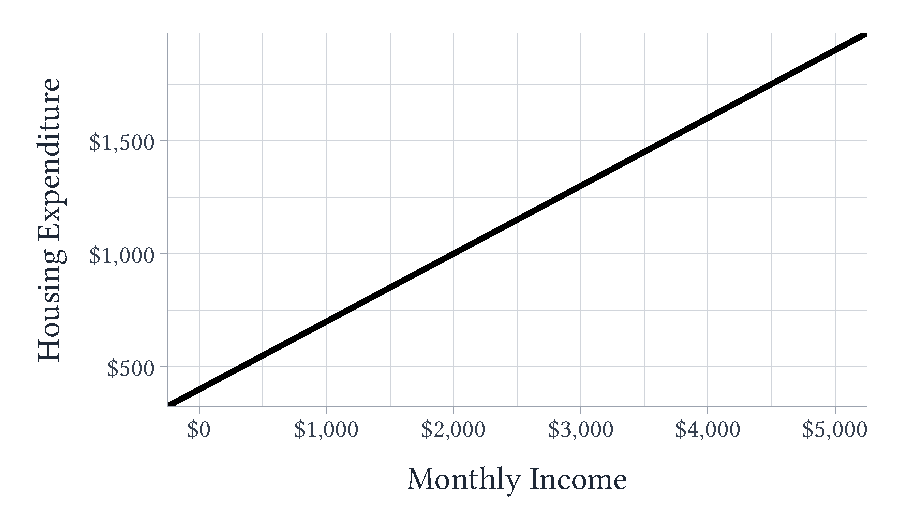
\includegraphics[width=0.8\textwidth]{figures/line_housing.pdf}
  \end{center}
\end{figure}

The first thing we can do is get predictions out for a specific income, say $\kelly{\$2500}$, by plugging it into our equation:
$$
  \text{Housing Expenditure} = 400 + 0.35 * \kelly{2500} = \$1275
$$
We call these \emph{fitted values} as you take the value of your explanatory variables and use the model fit to predict the value of the outcome variable (we will discuss this more later in the course). 

Also, we can think about changing someone's income and seeing how the outcome variable changes. Say you change from $x_1$ to $x_2$, how does $y$ change in response?
\begin{align*}
  y_2 - y_1 
  &= (\beta_0 + \beta_1 * x_2) - (\beta_0 + \beta_1 * x_1) \\
  &= \beta_1 (x_2 - x_1).
\end{align*}

We can write this more succinctly as $\Delta y = \beta_1 * \Delta x$, where $\Delta$ (greek for $D$ for ``difference'') takes the difference between the new and old values of the variable. Notice the slope plays an important role here. It tells us when you change $x$ by a certain amount, then $y$ changes by that amount \emph{scaled} by $\beta_1$. So, if I increase $x$ by one unit, then $y$ changes by $\beta_1$ units.

In our housing example, if I increase my income by $500$, then I change my housing expenditure by $0.35 * 500 = 175$ dollars.

\subsection*{Multiple variables}

Say we have the following $y = \beta_0 + \beta_1 x_1 + \beta_2 + x_2$, where $x_1$ and $x_2$ are two explanatory variables. Using simlar math above, show that 
$$
  \Delta y = \beta_1 \Delta x_1 + \beta_2 \Delta x_2
$$

Say we want to examine how $y$ changes when you change $x_1$ while holding $x_2$ equal (latin lesson, this is called `ceteris palabus' or `all else equal'). We have $\Delta x_2 = 0$, so $\Delta y = \beta_1 \Delta x_1$ just like before. 

As an example, think about predicting how many dollars a person will spend on a product given (i) the price of the product $p$ and (ii) the consumer's disposable income $I$. Let's say this is given by 
$$
  Q = 120 - 9.8 * p + 0.03 * I
$$

Say disposable income stays fixed at $\$900$ but the price increases from 8 to 9 dollars. How will the quantity demanded change?
\begin{align*}
  \Delta Q 
  &= -9.8 * \Delta p + 0.03 * \Delta I \\
  &= -9.8 * 1 + 0.03 * 0 = -9.8
\end{align*}

The quantity demanded will decrease by 9.8 units.


\section{Quadratic Functions}

Now say you model the relationship between $x$ and $y$ with a quadratic function
$$
y = \beta_0 + \beta_1 x + \beta_2 x^2
$$
Adding polynomial terms allows the relationship between $x$ and $y$ to not be linear. See figure \ref{fig:example_wage} for an example. The figure plots a linear relationship and quadratic relationship between age and wages. The quadratic equation better represents the facts that (i) workers are promoted more often at younger ages (quicker wage growth) and (ii) earnings peek around age 45 for workers.

\begin{figure}
  \caption{Linear vs. Quadratic functions}
  \label{fig:example_wage}
  \begin{center}
    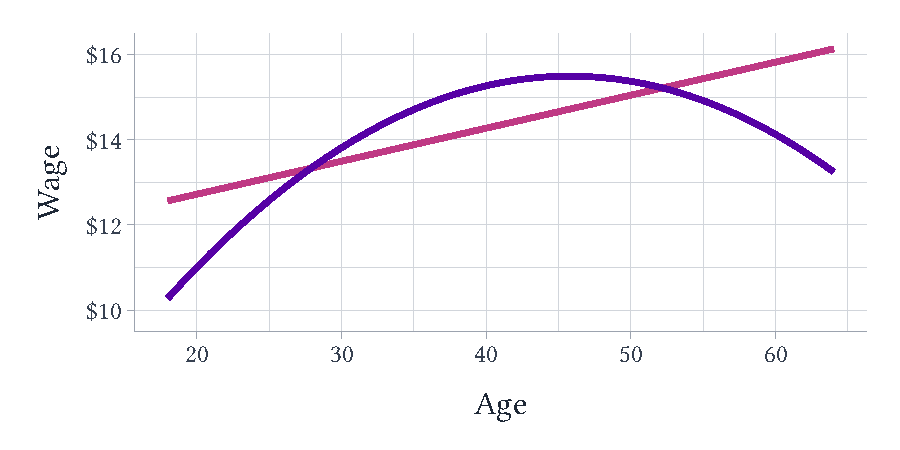
\includegraphics[width=0.8\textwidth]{figures/wage_models.pdf}
  \end{center}
\end{figure}

The equation for wages is given by 
$$
  \text{Wage} = -5.5 + 1 * \text{Age} - 0.01 * \text{Age}^2
$$

Given this equation, how do wages change as a person ages? We could do some algebra using the method before (or using derivatives), but I'll show you the answer:
$$
  \Delta \text{Wage} = \left( 1 - 2 * 0.01 * \text{Age} \right) \Delta \text{Age}
$$
The answer got more complicated, but that makes sense looking at the figure. Following the curve, the direction you move to stay on the line depends on where you are on the line (age). E.g. moving from 25 to 30, wages increase by $(1 - 2 * 0.01 * 25) * (30 - 25) = +\$2.50$. From 55 to 60, wages decrease by $(1 - 2 * 0.01 * 55) * (60 - 55) = -\$0.50$.

More generally, the formula is given by 
$$
  \Delta y = \underbrace{(\beta_1 + 2 * \beta_2 * x)}_{\text{depends on starting } x} * \Delta x 
$$


\section{\texorpdfstring{$\log$}{log} transformations}

Sometimes, we will talk about when in the course, it is beneficial to log either the outcome and/or explanatory variables. Log transformed variables change the interpretation of our linear regression lines. It takes from `unit changes' to `percent changes'. E.g. I could model $\log(\text{Wages})$ as a linear regression of age. My interpretation would be that increasing age by 1 year would increase wages by $\beta_1 * 100$ percent.

An example for how to interpret each combination of log and non-logged $y$ and $x$ variables is given in Table \ref{tab:log_transformations}.

\begin{table}
  \caption{Summary of log-transformed linear equations}
  \label{tab:log_transformations}

  \begin{tabular}{@{}
    p{0.3\textwidth} p{0.6\textwidth}
  @{}}
    \toprule
    \textbf{Model} & \textbf{Interpretation} \\

    \addlinespace[1mm]
    \midrule
    \addlinespace[1mm]

    $y = \beta_0 + \beta_1 x$ & 
    A 1 unit increase in $x$ increases $y$ by $\beta_1$ units \\

    $\log(y) = \beta_0 + \beta_1 x$ & 
    A 1 unit increase in $x$ increases $y$ by $\beta_1 * 100$ percent \\

    $y = \beta_0 + \beta_1 \log(x)$ & 
    A 1 percent increase in $x$ increases $y$ by $\beta_1$ units \\

    $\log(y) = \beta_0 + \beta_1 \log(x)$ & 
    A 1 percent increase in $x$ increases $y$ by $\beta_1 * 100$ percent \\

    \bottomrule
  \end{tabular}
\end{table}

For example, let's derive this for $y = \beta_0 + \beta_1 * \log(x)$. We have:
\begin{align*}
  \Delta y &= \beta_1 \left( \log(x_2) - \log(x_1) \right) \\
  &\approx \beta_1 * \frac{x_2 - x_1}{x_1} \\
  &= \beta_1 * \% \Delta \text{ in } x \\, 
\end{align*}
where the approximation holds for small changes in $\Delta x$ (think like a 1 percent increase). If you remember your high school science class, percent change is calculated (new - old / old) which is exactly what we have on the right hand side, the percent change in $x$. 

This derivation will work the same for the other equations as summarized in Table \ref{tab:log_transformations}. Just remember that if you have a $log$, then it is percent change.



\part{Review of Probability and Statistics}

\section{Single Random Variables}

There are two key concepts to understand. First, we have an \textbf{experiment} which is the source of \emph{randomness} in the world: e.g. flip a coin, roll a dice, play a basketball game, et cetera. The second definition is a \textbf{random variable}. A random variable assigns numerical values that is determined by an experiment (e.g. value of a die roll, assigning 1 to heads 0 to tails). For an experiment, there are many different random variables you could define. For a NBA game, random variables include the number of points scored; a variable who equals 1 if the home team won and 0 if the home team loses; the average height of players who play; etc. 

We denote random variables by upper case letters, usually $W$, $X$, $Y$,
and $Z$. The particular values that a random variable takes are denoted by the corresponding lower case letters $w$, $x$, $y$, and $z$.

For , think about a the coin-flipping experiment where you flip 10 coints. Let $X$ denote the random variable counting the number of heads that land out of the 10 flips. It is important to note $X$ is not associated with any particular value. You can do this experiment many different times and $X$ represents \emph{the process} of running the experiment, not the value of a particular trial. But, we know $X$ will take on a value in the set $\{ 0, 1, 2, \dots, 10 \}$, say $x = 6$ for a particular trial.


\subsection*{Discrete Random Variables}

When the random variable takes on \textbf{discrete} values (like $X$ above), the probability density function (pdf) assigns probabilities for $X$ obtaining any particular value. In the case of discrete values, this is sometimes called the probability mass function. Formally, say $X$ can take $n$ values. For all values, denoted by $x_j$, that the random variable can take, the pdf is defined as:
$$
  f_{X}(x_j) = \P{X = x_j} = p_j
$$

\begin{example}
  Say you flip a single coin and assign $X$ to equal 1 if the coin lands on heads and 0 if it lands on tails. The pdf for this random variable is $f(1) = 1/2$ and $f(0) = 1/2$.
\end{example}

There are two rules that the pdf must follow:
\begin{enumerate}
  \item For all values of $x_j$, $1 \geq f_{X}(x_j) \geq 0$ 
  \item $\sum_{j} f_{X}(x_j) = 1$
\end{enumerate}
In words, (1) says the probability $X$ takes a value $x_j$ has to be between 0 and 1, and (2) says the sum of the probabilities \emph{over all possible values} must equal 1 (i.e. something must happen).


The \textbf{cumulative distribution function} (cdf) is similar to the pdf but asks about the probability that $X$ takes a value less than or equal to some $x$:
$$
  F_{X}(x) = \P(X \leq x)
$$
Note that this means CDF must be (weakly) increasing in $x$ (e.g. $\P(X \leq 2)$ must be no larger than $P(X \leq 3)$). Also $0 \leq F_{X}(x) \leq 1$ must be true since that is true of probabilities.

\begin{example}
  Take a random variable, $Y$ with pdf of $p_1 = \P{Y = 1} = 0.2$, $p_2 = \P{Y = 2} = 0.5$, and $p_3 = \P{Y = 4} = 0.3$. Then, the CDF is given by 
  $$
    F_{y}(y) = \begin{cases}
      0.0   \quad \text{when } y < 1, \\
      0.2 \quad \text{when } 1 \leq y < 2, \\
      0.7 \quad \text{when } 2 \leq y < 4, \\
      1.0   \quad \text{when } y \geq 4, \\
    \end{cases}
  $$

  \qed
\end{example}

The probability density function is \emph{a complete picture} about a random variable; but it can often be too much information (imagine telling someone the probabilities for $X$ that can take the values $0$ to $100$.) While you could plot the pdf as a histogram, this still can be a lot of information. For that reason, we use \textbf{statistics} to `summarize a random variable'. 

\subsection*{Expectation}

The most common statistic we use is the mean, or in fancy words the `expectation'. A natural question we care about is `what is the average value of some random variable $X$?' For this, we use the \textbf{expectation} which takes the average of the values that $X$ can take weighted by how likely $X$ is to take that value:
$$
  \expec{X} \equiv \sum_{j=1}^n x_j \P(X = x_j) = \sum_{j=1} x_j p_j
$$

\begin{example}
  Take a random variable, $Y$ with pdf of $p_1 = \P{Y = 1} = 0.2$, $p_2 = \P{Y = 2} = 0.5$, and $p_3 = \P{Y = 4} = 0.3$. Then, the expectation is given by
  $$
    \expec{Y} = 1 * 0.2 + 2 * 0.5 + 4 * 0.3 = 2.4
  $$
  
  \qed
\end{example}

There are some properties of expectations that come out of the definitions of sums $\sum$:
\begin{enumerate}
  \item For any constant $c$, $\expec{c} = c$ (there's no randomness)
  \item For any constant $a$, $\expec{aX} = a \expec{X}$
  \item For any constant $a$ and $b$, $\expec{aX + bY} = a \expec{X} + b \expec{Y}$
\end{enumerate}

Lastly, we will discuss transformations of random variables. So for , say you have a function $g$ that takes the random variable, $X$, of the number of heads out of $10$ and assign to sum final score, $Y$. That is, $Y = g(X)$. The average value of $Y$ can be calculated using the pdf of $X$:
$$
  \expec{Y} = \expec{g(X)} = \sum_{j=1}^n p_j g(x_j)
$$

\subsection*{Variance}

The other most common statistic is the \textbf{variance} of a random variable. While the expectation tells you something about the `average' value you would observe the random value taking, the variance tells you something about the varaibility of the random variable. That is, how much does the random variable $X$ move around it's mean? A large variance means it moves around a lot.

The variance is given by 
$$
  \var{X} \equiv \expec{\left( X - \expec{X} \right)^2 } = \sum_j p_j (x_j - \expec{X})^2,
$$
where the last equality comes from the $g(X)$ rule we laid out above. 

The intuition around the variance is as follows. The value $x_j - \expec{X}$ tells you how far a particular $x$ value is from the expected value. If we just used the difference, then the positives ($x_j$ above the mean) and the negatives ($x_j$ below the mean) would cancel out which would make this a bad measure of variability. So, therefore, we square the term to make it positive everywhere.

Relatedly, the \textbf{standard deviation} is the square-root of the variance: 
$$
  \sd{X} \equiv \sqrt{\var{X}}
$$

In your own time, check the following using the definition of variance above:
\begin{enumerate}
  \item For any constant $c$, we have $\var{c} = 0$
  
  \item For any constants $a$ and $b$, $\var{aX + b} = a^2 \var{X}$
\end{enumerate}


\subsection*{Continuous Random Variables}

Now we turn to \textbf{continuous} random variables where random variables can take values on (parts of) the real number line (e.g. height). All our definitions and intuition still apply, but in continuous land, we basically move from sums $\sum$ to integrals $\int$. 

The probability density function is given by $f_{X}(x)$, but no longer represents the probability that $X$ obtains the value $x$. This is because with a continuum of values, the probability you obtain any \emph{particular} value becomes 0. E.g. what's the probability someone is \emph{exactly} 5 ft. 8.124028 in.?\footnote{As an aside, you might argue `well with a ruler we would round these variables to the nearest tenth of an inch', so isn't that discrete? I guess you can make this argument and treat it as a discrete variable, but it is better to think of these things as continuous (later in the class it will make the math simpler, not harder!) and we will in this class.}
Instead, it is better to think of the density function as giving a `relative likelihood' that you take a value ``near $x$''. More formally, the density function can tell you the probability you're in a range of values $[\ubar{x}, \bar{x}]$: 
$$
  \P{X \leq x} = \int_{\ubar{x}}^{\bar{x}} f_{X}(x) dx,
$$
This can be used for the CDF too:
$$
  \P{X \leq x} = \int_{-\inf}^x f_{X}(x) dx,
$$

Similarly, expectations still take the form of "the value times the density", but we `average' this using the integral:
$$
  \E{X} = \int x * f_{X}(x) dx.
$$
All the properties listed above hold for continuous variables too (or mixtures of both). 

Last, the variance is given by
$$
  \var{X} = \int (x - \expec{X})^2 f_{X}(x) dx
$$


\section{Multiple Random Variables}

In this class, we care about how variables relate to one another. For , do sales grow and shrink with a consumer's age?; is height an important predictor of basketball success?; is the sale associated with a large increase in sales?

For this, we would want to know about the \textbf{joint distribution} between two variables $X$ and $Y$. 

The \textbf{joint probability density function} is denoted by $f_{X,Y}(x, y)$. In the discrete case, it is the probability that $X = x$ \emph{and} $Y = y$ \emph{in the same trial}:
$$
  f_{X,Y}(x, y) = \P{X = x, Y = y}.
$$

We can also think about \textbf{conditioning} on the value of one of the random variables. That is, take $Y$ to be \emph{fixed} to some value $y$. Then we could ask about the distribution of $X$ \emph{within trials where $Y = y$}.
$$
  f_{X \vert Y}(x \vert y) = \P{X = x}{Y = y}
$$
Note we use the $\vert$ symbol to note `conditioning' on some random variable's realization. The things on the right we are conditioning on. In our , we learn that $Y = y$ for that trial and then ask about the (conditional) probability that $X = x$.

The \textbf{Bayes Rule} helps us translate between conditional pdfs and the joint pdfs:
$$
  f_{X \vert Y}(x \vert y) = f_{X,Y}(x, y) / f_{Y}(y).
$$
So say we have two discrete random variables and we want to know probability $X = x$ conditional on $Y = y$. We can calculate it if we know (1) the probability that $Y = y$ and (2) the joint probability that $Y = y$ \emph{and} $X = x$. 


\subsection*{Covariance and Correlation}

Similar to how we used statistics to summarize a single random variable, it is common to want to summarize how to variables are related to one another. For this we use the \textbf{covariance} or the \textbf{correlation} between two variables. They are very similar to one another.

The covariance looks like the variance of a random variable:
$$
  \cov(X, Y) = \mathbb{E}\left[ (X - \expec{X}) (Y - \expec{Y}) \right]
$$
The covariance intuitively measures whether $X$ and $Y$ move together. The covariance is positive if when $X$ is above it's mean, $Y$ also tends to be above it's mean and when $X$ is below it's mean, $Y$ also tends to be below it's mean. They ``co-move'' together.

The covariance is negative if when $X$ is above it's mean, $Y$ tends to be below it's mean and vice versa. They move in opposite directions, but are still related! In other words, if I know $X$ was above it's mean, then I would predict that $Y$ is below it's mean (knowing one gives me information on the other). 

With some algebra and the rules of expectations, we can see
\begin{align*}
  \cov(X, Y) 
  &= \mathbb{E}\left[ (X - \expec{X}) (Y - \expec{Y}) \right] \\
  &= \mathbb{E}\left[ XY - \expec{X} Y - X \expec{Y} + \expec{X} \expec{Y} \right] \\ 
  &= \expec{XY} - \expec{X} \expec{Y} - \expec{X} \expec{Y} + \expec{X} \expec{Y} \\
  &= \expec{XY} - \expec{X} \expec{Y}.
\end{align*}


The correlation is just a rescaled version of the covariance:
$$
  \corr(X, Y) = \frac{\cov(X, Y)}{\sd{X} \sd{Y}}.
$$
The correlation is designed to always be between -1 and 1 (because of the rescalling), so it is more popular since people are used to thinking about correlations. A correlation close to 1 and/or -1 is a \emph{very strong} relationship. 

It is important to know that covariance and correlation only measure a \emph{linear} relationship between $X$ and $Y$; if the function connecting $X$ and $Y$ is non-linear, then the correlation is a bad summary statistic of the corelationship between them. This is similar to how the mean is a bad measure for highly skewed data.

\subsection*{Independence}

Two random variables are said to be \textbf{independent} if knowing information about the realization of one of them tells you nothing about the realization of the other one. That is, if I told you the day was sunday ($X = $ Sunday), then you would not have any better prediction about whether it is raining ($Y = 1$). The two random variables are independent. 

When $X$ and $Y$ are indepedent, this can be summarized by $f_{X \vert Y}(x \ \vert \ y) = f_{X}(x)$. This also implies that when $X$ and $Y$ are independent,
$$
  F_{X,Y}(x, y) = F_{X}(x) F_{Y}(y).
$$

Using the definition of expectations, we can derive the following when $X$ and $Y$ are independent:
\begin{itemize}
  \item $\expec{XY} = \expec{X} \expec{Y}$
  \item $\cov(X, Y) = 0$
  \item $\var{aX + bY} = a^2 \var{X} + b^2 \var{Y}$
\end{itemize}

The last fact comes from the fact that for \emph{all} random variables $\var{aX + bY} = a^2 \var{X} + b^2 \var{Y} + 2ab \cov(X, Y)$, but the last term is zero from independence.


\section{Normal Distribution}

The normal distribution is one of the most important distributions in statistics. When a variable is normally distributed, we write $X \sim \mathcal{N}(\mu, \sigma^2)$, where $\mu = \expec{X}$ and $\sigma^2 = \var{X}$. The normal distribution is symmetric and the density function of the normal distribution looks like a `bell'. The parameter $\mu$ changes where the center of the distribution is and $\sigma^2$ determines how wide the distribution is.


See the figure for example: 
\begin{figure}
  \caption{Example PDFs for different Normal Distributions}
  \begin{center}
    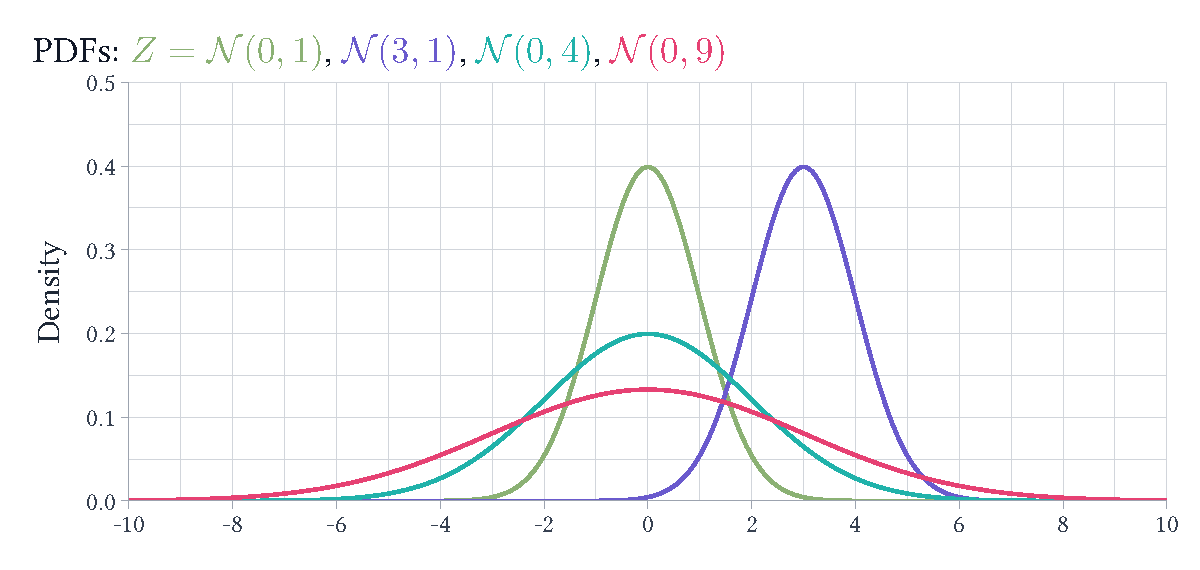
\includegraphics[width=0.8\textwidth]{figures/ex_normal_dist.pdf}
  \end{center}
\end{figure}


We can calculate probabilities of taking values $X \in [\ubar{x}, \bar{x}]$ by integrating the area under the pdf. The pdf is given by
$$
  f_X(x) = \frac{1}{\sigma\sqrt{2\pi}} \exp\left( -\frac{1}{2}\left(\frac{x-\mu}{\sigma}\right)^{\!2}\,\right).
$$
Would you want to integrate this function? My guess is probably not. 

Instead, we refer to the $Z$-table which calculates probabilities for the \textbf{standard normal distribution} denoted $Z = \mathcal{N}(0, 1)$. It then calculates $P(Z \leq z)$ for values of z ranging from $-3$ to $3$. Since we do not have a \emph{standard} normal distribution, we can \textbf{standardize} our variable $X$ to make it standard normal:
$$
  \frac{X - \mu}{\sigma} \sim Z = \mathcal{N}(0, 1)
$$

\begin{example}
  Say we have $X \sim \mathcal{N}(10, 4)$ and we want to know $\prob{X \leq 12}$. Then we can standardize our problem:
  $$
    \prob{X \leq 12} = \prob{\frac{X - 10}{2} \leq \frac{12 - 10}{2}} = \prob{Z \leq 1} 
  $$

  The last probability we can find in our $Z$-table by looking up the z-score of $1$. 

  \begin{figure}[h!]
    \begin{center}
      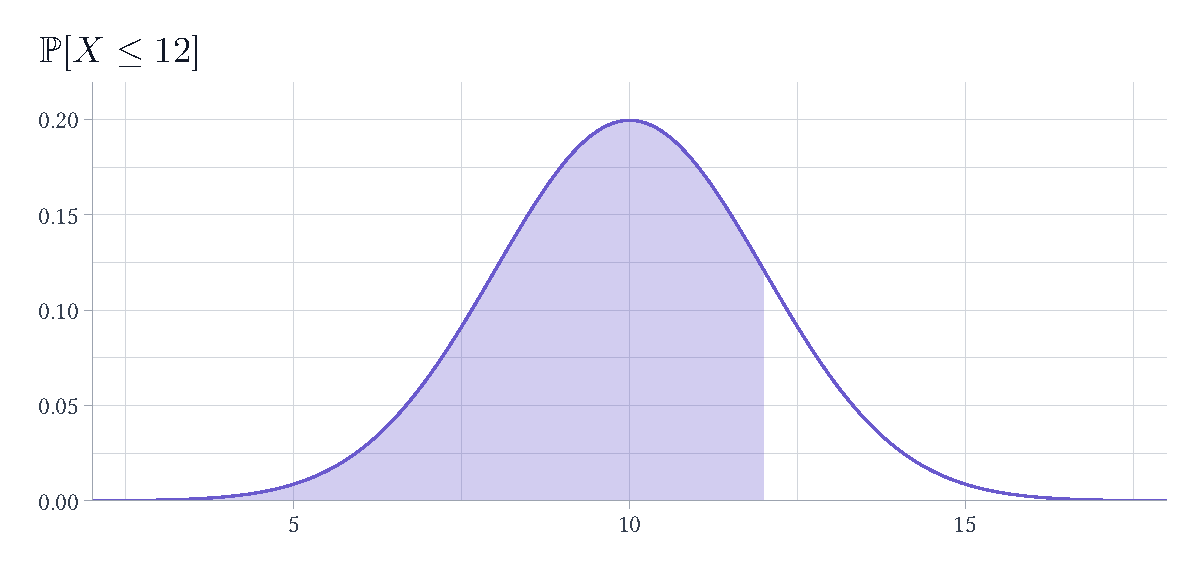
\includegraphics[width=0.75\textwidth]{figures/ex_probability_leq.pdf}
    \end{center}
  \end{figure}

  Moreover, arbitrary intervals like $[\ubar{x}, \bar{x}]$ can be calculated as $\prob{X \leq \bar{x}} - \prob{X \leq \ubar{x}}$.

  \begin{figure}[h!]
    \begin{center}
      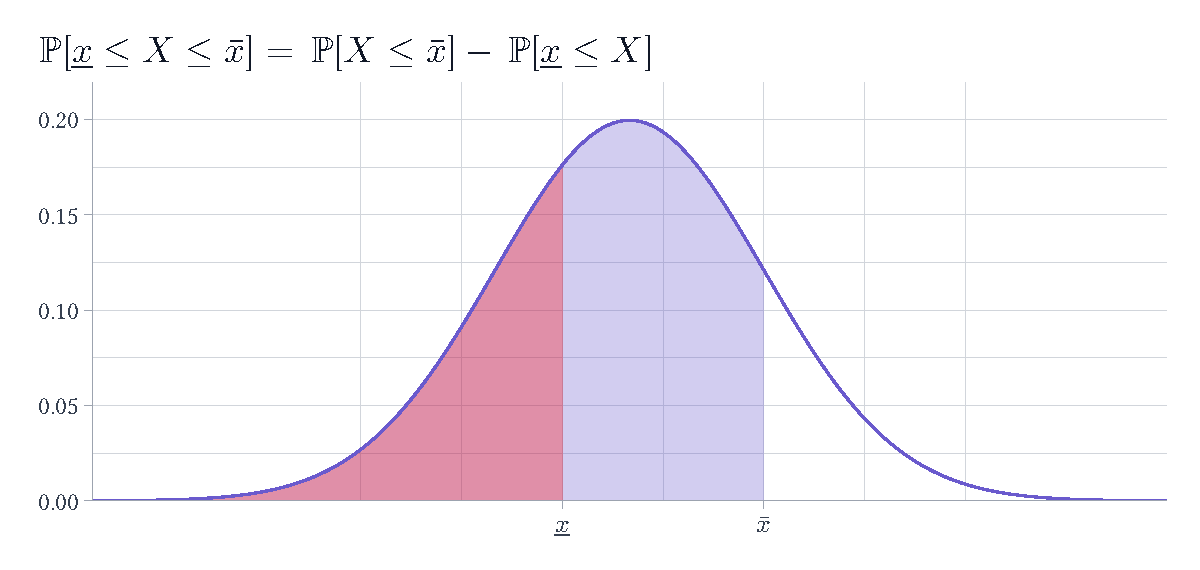
\includegraphics[width=0.75\textwidth]{figures/ex_probability_between.pdf}
    \end{center}
  \end{figure}
  
  \qed
\end{example}


\subsection*{The 68-95-99.7 rule}

With the normal distribution, we have the 68-95-99.7\% rule which says that 68\% of observations drawn from a $\mathcal{N}(\mu, \sigma^2)$ random variable will be within the range $\left[\mu - \sigma, \mu + \sigma\right]$ (within one standard deviation from the mean); 95\% will fall within two standard deviations from the mean; and 99.7\% will fall within three standard deviations. In figure form: 
\begin{figure}[h!]
  \begin{center}
    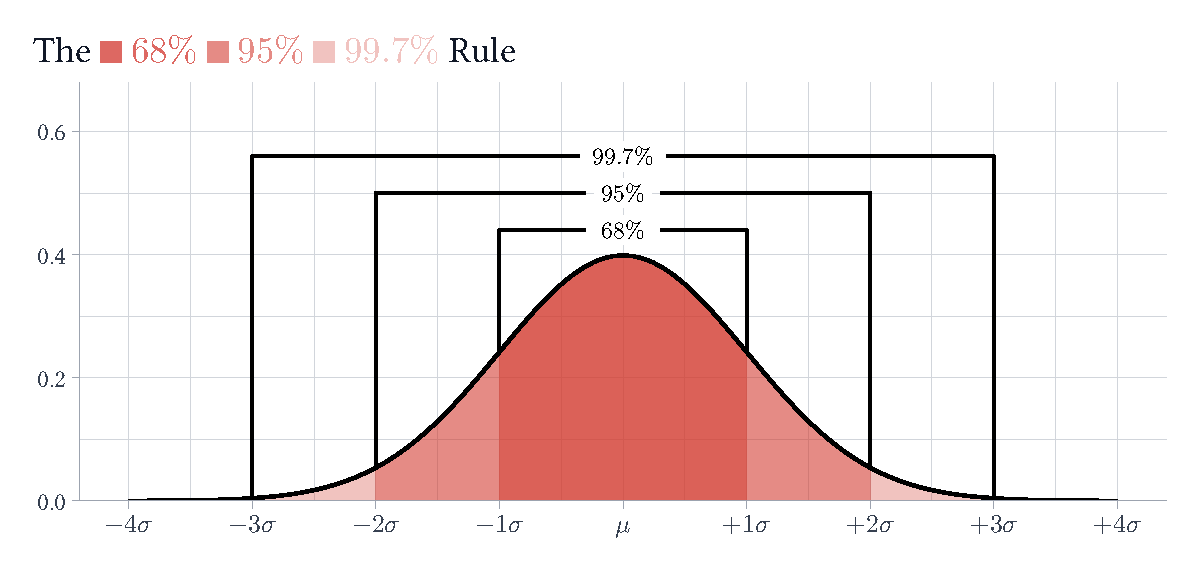
\includegraphics[width=0.9\textwidth]{figures/68_95_99.pdf}
  \end{center}
\end{figure}







\section{Statistical Inference}

\textbf{Statistical Inference} is the procedure of using a random sample of observations from a population to try and learn something about the population distribution of the data. To be more specific, there is some \emph{statistic} of the population distribution (e.g. it's expectation, it's variance, the 80th percentile, etc.) that we want to know about. Let's call that statistic $\theta$. 

\subsection*{Estimators}

We do not observe the full population; only just a sample. We take our random sample, $X_1, \dots, X_n$, and want to \textbf{estimate} the population statistic. We calculate an \textbf{estimate} of the population statistic using the data. The calculation we chose to make is called our \textbf{estimator}. For , we can use the sample average from a set of observations to infer about the expectation of the population. To do so, we could calculate the sample average of our sample:
$$
  \underbrace{\bar{X}}_{\text{Estimator}} \equiv 1/n \sum_{i=1}^n X_i
$$

Any particular way to estimate the population statistic is called a \textbf{estimator}. For any statistic, there are many different estimators. Therefore, we have some ways to discuss what makes a good estimator.

\textbf{Property 1: \textbf{Unbiasedness}} 

We say an estimator $W$ is an unbiased estimator for $\theta$ if:
$$
  \expec{W} = \theta.
$$
That is, if we take a bunch of random samples (\textbf{repeated sampling}) and averaged them, on average the estimator would equal the population statistic.

Note this is not saying the estimate always equals the population statistic, just that on average it does. For , the sample mean does not always equal the population mean, but it is an unbiased estimate for the population mean.

\textbf{Property 2: \textbf{Consistency}}

Let $W_n$ be an estimator of $\theta$ based on a population of size $n$. The estimator is consistent if as $n$ gets larger, $W_n \to \theta$ and the variance of $W_n$ shrinks to 0. That is, the estimator gets more precise and centers around the population statistic.

\textbf{Property 3: \textbf{Efficiency}}

If $W_1$ and $W_2$ are two unbiased estimators, we say $W_1$ is more efficient than $W_2$ if $\var{W_1} < \var{W_2}$.


\subsection*{Confidence Intervals}

Since the estimator does not always equal it's population statistic (in repeated sampling) We want to be able to describe the uncertainty of an estimator. To do so, we need to have an estimate to the variability of our estimator in repeated sampling. 

That is, we want to quantify how much we think our estimator would move around if we were to collect a bunch of different samples of the same size and calculate the estimator for each sample. This thought experiment of grabbing a bunch of samples of the same size and calculating our estimator on each sample creates what we call our \textbf{sample distribution} of our estimates. 


It turns out that for a lot of estimators, the sample distribution is approximately \textbf{normally distributed}. That makes summarize our uncertainty around our estimator easier. We typically will construct a \textbf{confidence interval} to descirbe our level of certainty. The confidence interval is centered on our estimate, but it's width describes a range of values we think the population statistic could be. 

\begin{example}
  Let $\{ Y_1, \dots, Y_n \}$ be a random sample. The sample mean is approximately distributed $\mathcal{N}(\mu, \sigma^2 / n)$ where $\mu = \expec{Y}$ and $\sigma^2 = \var{Y}$. 

  We can construct a 95\% confidence interval as: 
  \begin{align*}
    &\P{-1.96 < \frac{\bar{Y} - \mu}{\sigma / \sqrt(n)} < 1.96} = 0.95 \\
    \implies &\P{\bar{Y} - 1.96 * \frac{\sigma}{\sqrt(n)} < \mu  < \bar{Y} + 1.96 \frac{\sigma}{\sqrt(n)}} = 0.95
  \end{align*}

  That is, in repeated sampling, there is a 95\% probability (95 out of 100 samples of size $n$) that $\mu$ falls within our confidence interval: 
  $$
    \left[
      \bar{Y} - 1.96 * \frac{\sigma}{\sqrt(n)}, 
      \bar{Y} + 1.96 * \frac{\sigma}{\sqrt(n)}
    \right]
  $$
  Since we do not observe $\sigma$, we will estimate it using the following estimator, called the sample standard deviation of $y$:
  $$
    s = \sqrt{\frac{1}{n-1} \sum_{i=1}^n (Y_i - \bar{Y})^2}
  $$
\end{example}

In the above procedure, the values $-1.96$ and $1.96$ are the critical values for the 2.5th percentile and 97.5th percentile of the standard normal distribution, i.e. we have the middle 95\%. If we want to be more confident in our interval, then we need to use larger critical values. For , if we want to be 99\% confident in our interval (have $\theta$ in our interval in 99 out of 100 samples), then we need to use the 0.5th percentile and 99.5th percentile of the normal distribution for our critical values.

Note this procedure works because $\bar{Y} \sim \mathcal{N}(\mu, \sigma^2/n)$ and therefore our \textbf{$Z$-score}, $\frac{\bar{Y} - \mu}{\sigma / \sqrt(n)}$, is approximately distributed as the standard normal distribution.


\subsection*{Hypothesis Testing}

In addition to confidence intervals, it is common to perform \textbf{hypothesis tests}. Simply put, we want to test whether evidence is consistent with a \textbf{null hypothesis} that $\theta$ equals some value (e.g. we could hypothesize that the population mean height is 5 ft. 8 in.). We then would calculate our sample mean and if it is ``too far'' from the null hypothesis population mean, then we say the evidence rejects the null hypothesis. 

How far is ``too far'' away from the null hypothesis? That depends on (1) how noisy our estimate is (the sample distribution) and (2) how confident we want to be in rejecting the null. 

When I said before that we will see if our sample mean is ``too far'' away from the null, that was a little bit incorrect. For reasons we will not cover, we will transform the sample mean into a \textbf{test statistic}. When we compute the statistic for a particular outcome, we obtain an outcome of the test statistic, which we will denote $T$. 

\emph{When the null hypothesis is true}, the test statistic will be distributed as $\mathcal{N}(0, v)$ (normally distributed with mean $0$ and some variance $v$). Therefore, we expect $T$ to be very close to zero (if the null is true). So, if we find a value of $T = t$ that is ``very far'' away from zero, then we find evidence against the null hypothesis. 

Given a level of confidence (e.g. 95\%) and the variance $v$, we can use properties of the normal distribution to determine the probability that a draw from the $\mathcal{N}(0, v)$ distribution would be $\geq \abs{\hat{t}}$. This is called the \textbf{$p$-value}. In words, the $p$-value tells us, assuming the null hypothesis is true, how often would we expect to see a value as large or larger than the one we \emph{did observe in our sample}. If that probability is small, then we will reject the null.

In particular, given our level of confidence (e.g. 95\%), define the \textbf{significance level} as $\alpha = 1 -$ the level of confidence (e.g. 5\%). We reject the null if the $p$-value, $p$ is smaller than the level of confidence. Typically, we will use $\alpha = 0.05$. 

\begin{example}
  Let $\{ Y_1, \dots, Y_n \}$ be a random sample. The sample mean is approximately distributed $\mathcal{N}(\mu, \sigma^2 / n)$ where $\mu = \expec{Y}$ and $\sigma^2 = \var{Y}$. 

  We will test the null hypothesis $H_0: \mu = \mu_0$ for some proposed value $\mu_0$.

  Then, our test statistic is given by 
  $$
    T = \frac{\bar{X} - \mu_0}{\hat{\sigma} / \sqrt(n)},
  $$
  where $\hat{\sigma}$ is the square root of our estimate of the variance of $Y$. Assuming the null hypothesis is true, $H_0$, then $T \sim \mathcal{N}(0, 1)$.

  Therefore, the $p$-value is given by
  $$
    p = \prob{T \geq \abs{t}} = 2 * \prob{Z \leq -\abs{t}},
  $$
  where $Z$ is the standard normal random variable. 

  You can find this probability by looking up $-\abs{t}$ in the $Z$-table.

  \qed
\end{example}

Last, we will discuss the \textbf{rejection region} for a given \emph{null hypothesis}. This is defined as the set of values of our estimate where we would reject the null hypothesis for a given significance level, $\alpha$. 

\begin{example}
  Let $\{ Y_1, \dots, Y_n \}$ be a random sample. The sample mean is approximately distributed $\mathcal{N}(\mu, \sigma^2 / n)$ where $\mu = \expec{Y}$ and $\sigma^2 = \var{Y}$. 

  We will test the null hypothesis $H_0: \mu = \mu_0$ for some proposed value $\mu_0$.

  The rejection region can be found, most simply, by forming a confidence interval around the null hypothesis. Any value \emph{outside this interval} will be rejected.

  Our confidence interval for $\alpha = 0.05$ is given by 
  $$
    \left[ \mu_0 - 1.96 * \sigma/\sqrt{n},  \mu_0 + 1.96 * \sigma/\sqrt{n} \right]
  $$

  Therefore our rejection region is $\bar{X} \leq \mu_0 - 1.96 * \sigma/\sqrt{n}$ or $\bar{X} \geq \mu_0 + 1.96 * \sigma/\sqrt{n}$.

  \qed
\end{example}



\subsection*{Review}

In the population of cities granted enterprise zones in a particular state, let $Y$ denote the percentage change in investment from the year before to the year after a city became an enterprise zone. Assume that $Y$ has a $\mathcal{N}(\mu, \sigma^2)$ distribution.
\begin{itemize}
  \item State the null hypothesis that enterprise zones have no effect on business investment $\theta$ State the alternative hypothesis that they have a positive effect

  \item Suppose that the sample yields $\bar{Y} = 8.2, s = 23.9$ and $n = 36$. Construct and calculate the test statistic. Do you reject the null?

  \item What is the rejection region for a 5\% significance level?
\end{itemize}


% TODO: Add figures for the different inference tasks (e.g. p-value)




\end{document}
